\documentclass{../../text-style}

\texttitle{Лекция 1: Введение в робототехнику}

\begin{document}

\maketitle
\thispagestyle{empty}

\section{Введение}

Робототехника --- это наука об автономных технических системах, точнее, наука о разработке и применении роботов.
Правда, что такое автономные технические системы или роботы, консенсуса особого нет.
Вообще, слово \enquote{Робот} использовал ещё Карел Чапек в 1920-м году, в своей пьесе \enquote{Россумские универсальные роботы}, ещё когда даже компьютеров не существовало.
Под роботами обычно понимаются \enquote{автоматические устройства, предназначенные для осуществления различного рода действий, обычно выполняемых человеком}%
\footnote{Определение из Википедии, URL: \url{https://ru.wikipedia.org/wiki/Робот} (дата обращения: 08.02.2024).}%
, однако это вызывает больше вопросов, чем ответов. Например:

\begin{itemize}
    \item почтовый робот --- это автономная и, очевидно, техническая система, но всё-таки не то, про что будет речь в этом курсе;
    \item игрушки роботы-собаки не делают действий, обычно выполняемых человеком, но скорее роботы, чем нет;
    \item посудомойка --- автоматическое устройство, которое моет посуду, но не робот.
\end{itemize}

Мы, следуя традициям кибернетиков СПбГУ, будем называть роботами автономные автоматические устройства с замкнутым циклом управления с обратной связью, то есть устройства, способные действовать без участия человека (замкнутость цикла управления) и реагировать на изменения во внешней среде (обратная связь).
Обратите внимание, что, например, робот-сапёр с дистанционным управлением по нашему определению роботом не является, поскольку требует человека в контуре управления.
Однако это тоже не то чтобы точное определение, потому что, например, насосная станция поддерживает давление в водопроводе без участия человека, но не робот (а автомат).
Но думаю, что идея понятна, тем более что в этом курсе речь пойдёт прежде всего про мобильные роботы, в этой сфере понятие робота более определённо.

Кстати, насчёт кибернетиков.
\emph{Кибернетика} в общем смысле --- наука об управлении, изучает законы управления, взаимодействие управляющей и управляемой систем, информационные потоки и т.д. и т.п.
Это раздел прикладной математики, который имеет весьма опосредованное отношение к инженерии и, на самом деле, даже к робототехнике, поскольку кибернетика вполне применяется в таких нематериальных вещах, как экономика.
Кибернетикой мы в этом курсе заниматься не будем (только чуть-чуть коснёмся), но вообще на матмехе СПбГУ есть аж две кафедры кибернетики (теоретической и прикладной), с очень давней и очень славной историей, напрямую связанной с робототехникой (что интересно, робототехникой в основном занимаются как раз теоркибернетики).

\subsection{Какие роботы бывают}

Немного поговорим про типы роботов, используемые в разных областях народного хозяйства. 
Вообще, их можно разделить на два крупных класса --- стационарные роботы (манипуляторы) и мобильные роботы.

Как ни странно, в промышленности в основном используются именно стационарные роботы, то есть идеи писателей-фантастов про железных человекоподобных рабов, которые в конечном итоге восстают и уничтожают человечество, не нашли пока практического применения.
Реальный промышленный робот --- это манипулятор, намертво привинченный к полу, например, популярная серия роботов-манипуляторов KUKA:

\begin{center}
    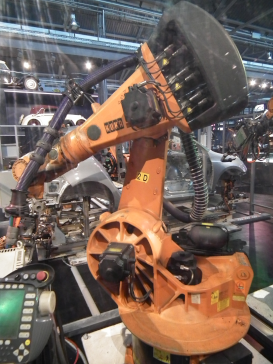
\includegraphics[width=0.5\textwidth]{kuka.png}
\end{center}

Несмотря на невпечатляющий внешний вид, это вполне робот, то есть автономная система, имеющая датчики и способная реагировать на изменения в окружающей среде.
В промышленных применениях основное изменение окружающей среды, на которое надо реагировать --- это появление препятствия в рабочей зоне (например, человека, которого желательно не зашибить, хотя для этого рабочую зону обычно просто огораживают).
Такие роботы используются в самых разных технических процессах, начиная от нанесения покрытия на деталь (когда её надо в течение пары десятков часов с равномерной скоростью вытягивать из раствора, на что человек в принципе не способен) заканчивая привинчиванием колёс к автомобилю.

Вот несколько более странно выглядящий робот-манипулятор:

\begin{center}
    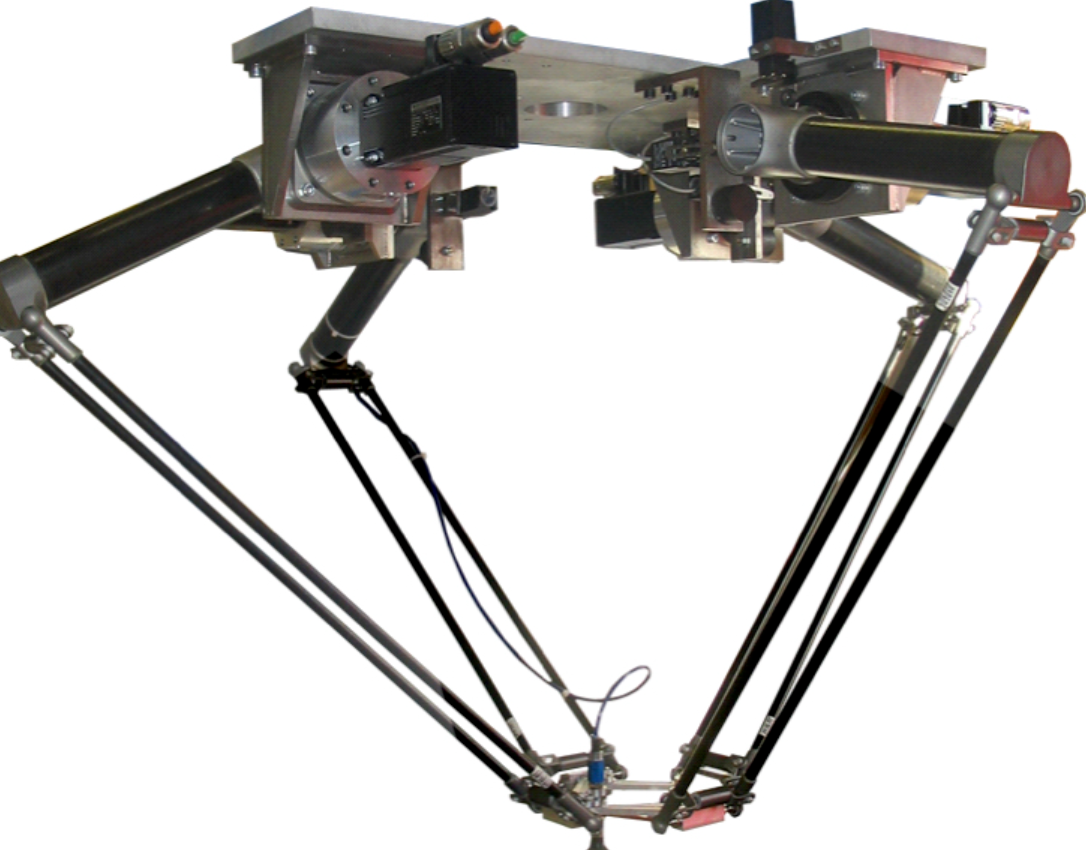
\includegraphics[width=0.5\textwidth]{delta.png}
\end{center}

Это один из так называемых дельта-роботов, которые хороши тем, что могут точно позиционироваться в трёхмерном пространстве, поэтому используются в точных производствах, например, монтаже печатных плат.
На них также есть датчики, которые часто используются для точного измерения пространственного положения манипулятора и его корректировки.

В этом курсе больше внимания будет уделено мобильным роботам.
Они тоже делятся на целый ряд сильно непохожих друг на друга типов:

\begin{itemize}
    \item Колёсные или гусеничные --- от робота-пылесоса до марсохода, широко используются и в промышленности (складские роботы), и в быту, стандарт де-факто в научных работах по робототехнике в силу простоты, практичности и эффективности.
    Беспилотные автомобили тоже попадают в эту категорию.
    \item БПЛА --- новый тренд в робототехнике, используемый в военном деле, сельском хозяйстве, для обнаружения лесных пожаров, контроля состояния трубопроводов, построения карт и трёхмерных моделей местности и т.д. и т.п.
    В основном сейчас распространены дистанционно управляемые беспилотные аппараты, которые, несмотря на развитую автоматику для поддержания положения в пространстве, роботами в смысле этого курса назвать нельзя.
    Однако среди БПЛА встречаются и роботы в самом полном смысле этого слова, БПЛА также любимы учёными-робототехниками за \sout{возможность записывать впечатляющие видео по групповому взаимодействию беспилотников} отличную мобильность и огромную потенциальную полезность в хозяйстве.
    БПЛА в свою очередь делятся на:
    \begin{itemize}
        \item аппараты условно вертолётного типа --- квадрокоптеры, гексокоптеры и т.п.; тогда как настоящие вертолёты (то есть аппараты с автоматом перекоса) используются крайне редко в силу сложности и дороговизны требуемой механики;
        \item аппараты с фиксированным крылом (к ним же в целом можно отнести конвертопланы).
    \end{itemize}
    Квадрокоптеры дёшевы, просты и очень мобильны, но ограничены в автономии, аппараты с фиксированным крылом могут хоть бесконечно находиться в воздухе (см., например, Airbus Zephyr).
    Кстати, современные (и не очень) крылатые ракеты вполне можно считать роботами --- навигация по рельефу местности в них была реализована ещё в 70-х годах 20-го века (см. BGM-109 \foreignquote{english}{Tomahawk}).
    \item Надводные и подводные роботы --- по задачам и особенностям управления весьма схожи с БПЛА, но имеют гораздо более узкую сферу применения.
    \item Шагающие роботы --- эффектны (см. роботы Boston Dynamics), способны работать на пересечённой местности, но очень сложны в управлении и довольно неэффективны.
    На практике особо не применяются, хотя R. Siegwart в своей книге приводит вот такую штуку для лесозаготовок:
    \begin{center}
        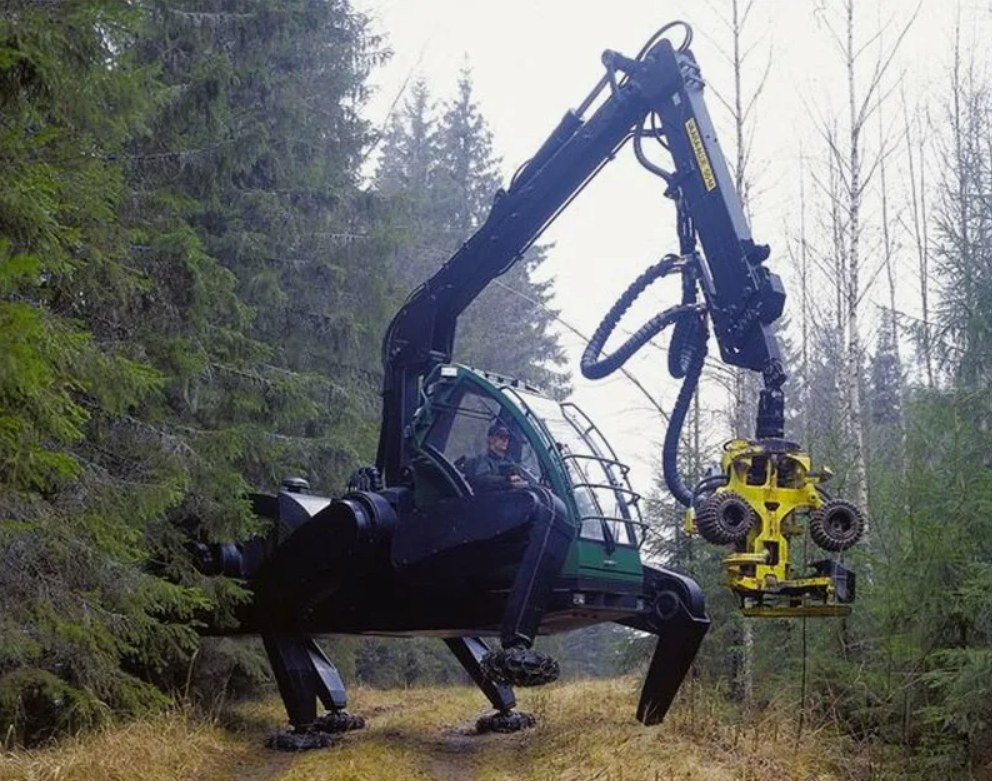
\includegraphics[width=0.5\textwidth]{plustechWalker.png}
    \end{center}
    Это не робот в нашем понимании, поскольку требует оператора (хотя сам управляет ногами), но шагающий и якобы полезный, поскольку может двигаться в непролазных чащобах, где у колёсной и даже гусеничной техники нет шансов.
\end{itemize}

\subsection{Робототехника на матмехе}

На матмехе робототехникой занимаются давно и довольно успешно, также вокруг матмеха есть довольно много сильных команд в этой области, занимающихся исследованиями вполне мирового уровня.
Для чего, собственно, и проводится этот курс --- дать обзор, ввести в курс дела, заинтересовать, чтобы в магистратуре можно было к этим исследованиям присоединиться.
Чем занимались (и занимаются) на матмехе в плане робототехники:

\begin{itemize}
    \item Образовательный конструктор ТРИК для обучения робототехнике и основам программирования школьников и студентов.
    Разрабатывался скорее \enquote{вокруг} матмеха, отдельной компанией, где не все были матмеховцами, но начиналось всё из коллаборации преподавателей кафедры теоретической кибернетики и системного программирования, и они же всегда были главной движущей силой проекта.
    Конструктор ТРИК широко известен в школьной робототехнике, признан как официальный для ряда олимпиад, используется в школьном образовании и в зарубежье.
    Вот пример робота-тележки ТРИК:
        \begin{center}
            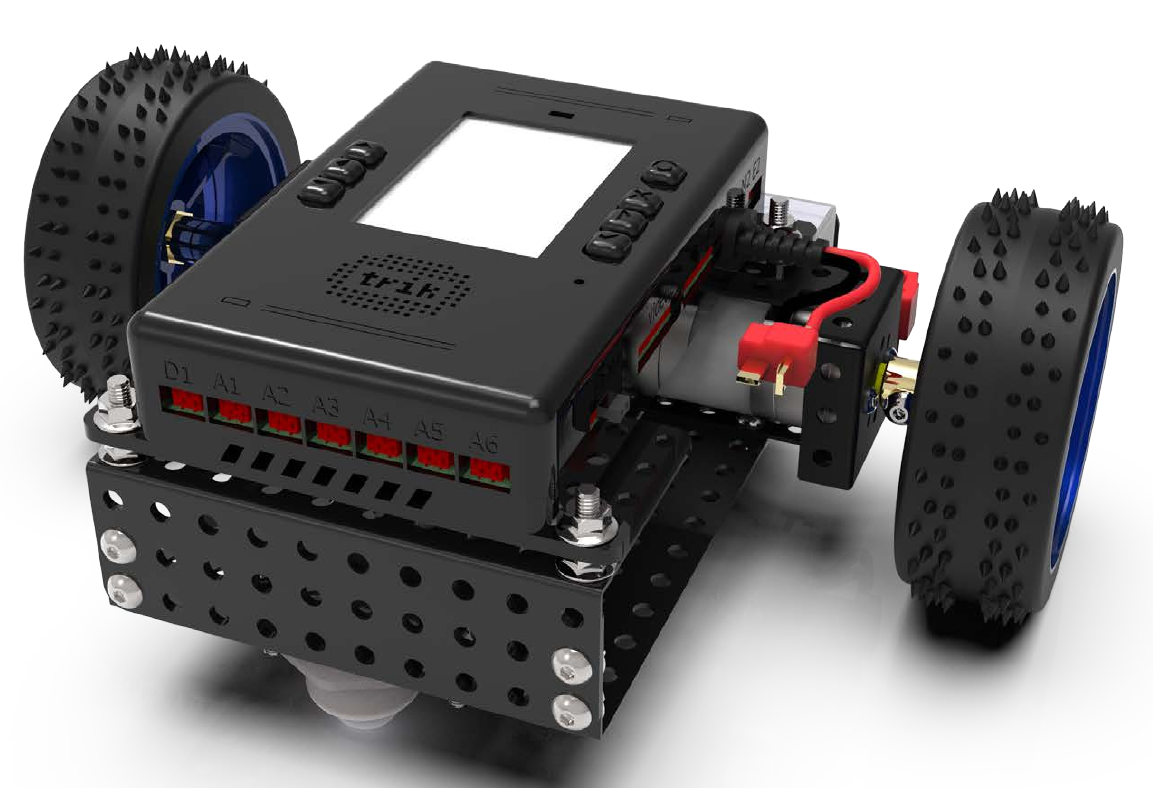
\includegraphics[width=0.6\textwidth]{trik.png}
        \end{center}
    \item Среда программирования TRIK Studio/QReal:Robots --- визуальная система программирования для образовательной робототехники, изначально создавалась для конструктора Lego Mindstorms NXT, потом там появилась поддержка Lego Mindstorms EV3 и ТРИК, потом и ряда других конструкторов.
    Тоже пошла в народ, тоже признана как официальная среда программирования на олимпиадах, на её основе записано вроде как несколько онлайн-курсов (для Stepik), защищена одна диссертация.
    \item Ресурсный центр \enquote{Робототехника и БАС} --- недавно созданный ресурсный центр СПбГУ, тоже не совсем на матмехе, там занимаются в основном беспилотниками.
    \item Кафедра теоретической кибернетики профессионально занималась робототехникой ещё до того, как все мы родились, причём занималась не только фундаментальной наукой, но и строила свои роботы.
\end{itemize}

\section{Алгоритмические основы}

Этот курс в называется \enquote{Алгоритмические основы робототехники}, поэтому с алгоритмических основ и начнём.
Алгоритмы в роботах нужны для управления, в самом широком смысле, от управления моторами до планирования миссии.
Управление в целом работает по стандартной схеме, описываемой архитектурным шаблоном \enquote{Sense-Compute-Control}:

\begin{center}
    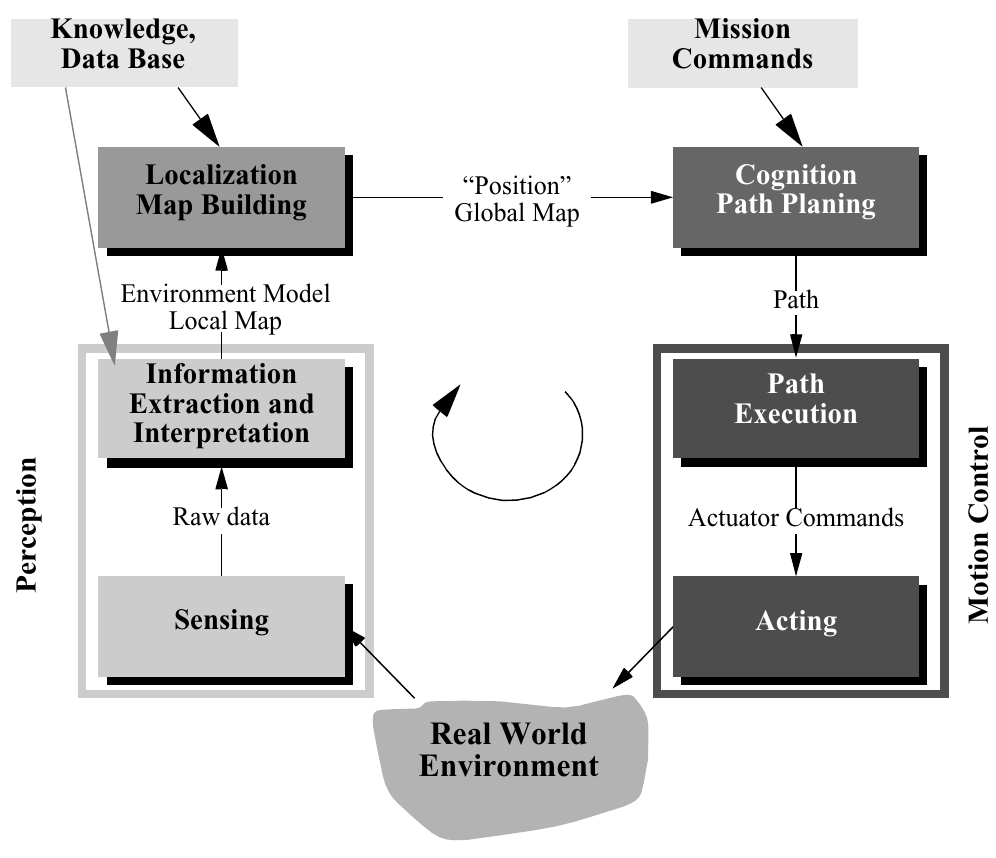
\includegraphics[width=0.7\textwidth]{controlLoop.png}
    \attribution{R. Siegwart, I.R. Nourbakhsh, Introduction to Autonomous Mobile Robots}
\end{center}

Реальный мир воспринимается сенсорами, из их показаний извлекается и интерпретируется информация.
Это на самом деле важный и нетривиальный этап работы бортового программного обеспечения --- коллеги с кафедры теоретической кибернетики приводили аналогию, что робот похож на человека, сидящего в бочке, и вынужденного по числам, показываемым приборами, строить картину мира вокруг.
Дальше, если это требуется, выполняется локализация или какой-то другой метод понять, в каком состоянии мы сейчас находимся.
Дальше, принимая во внимание поставленную задачу, мы должны понять, что именно надо делать дальше --- например, проложить маршрут к целевой точке.
По проложенному маршруту мы должны рассчитать управляющие воздействия на \emph{актуаторы} --- устройства, которые могут воздействовать на окружающий мир, например, двигатели моторов.
Ну и, наконец, обеспечить подачу рассчитанных управляющих воздействий до следующей итерации цикла управления.
При этом робот взаимодействует с реальным миром (например, перемещается в нём), действия робота приводят к ответной реакции реального мира, которая в свою очередь воспринимается сенсорами робота (результат перемещения --- изменение показаний камер или дальномеров, например).

Принципиальное отличие от программного обеспечения тут в том, что цикл управления вынужден взаимодействовать с реальным миром, который вообще плохо поддаётся оцифровке и алгоритмизации.
Сенсоры неизбежно шумят и врут.
Актуаторы неизбежно отрабатывают не точно.
При локализации неизбежны ошибки, причём они могут быть весьма значительными и приводить к весьма неприятным последствиям%
\footnote{См., например, известный инцидент, когда из-за навигационной ошибки в 1991 году американские вертолёты открыли огонь по своим: \url{https://www.govinfo.gov/content/pkg/GAOREPORTS-OSI-93-4/html/GAOREPORTS-OSI-93-4.htm} (дата обращения: 09.02.2024). Это были не роботы, но навигация для роботов ещё сложнее.}.
И реальный мир имеет свойство изменяться как в ответ на действия робота, так и сам по себе --- например, в окружении робота может быть много подвижных объектов, которые по показаниям сенсоров очень сложно отличить от стационарных, так что построение карты оказывается очень нетривиальной задачей.

Поэтому для роботов необходимы сложные алгоритмы управления.
Но начнём мы с простых.

\subsection{Регуляторы}

В самых простых ситуациях управление сводится к формальной математической задаче: имея установочное значение (то есть, например, желаемое показание датчика), вырабатывать управляющее воздействие (то есть, например, мощность, которую нужно подавать на моторы) так, чтобы система оставалась к установочному значению как можно ближе.
Пример такой задачи --- езда вдоль стены робота, когда мы фиксируем расстояние до стены, которое робот должен поддерживать, и он едет вдоль, не сильно от установленного расстояния отклоняясь.
Или круиз-контроль в автомобиле --- задаём желаемую скорость, автомат поддерживает обороты двигателя так, чтобы автомобиль с этой скоростью двигался, не важно, по прямой или в гору.
Или авиационный автопилот, поддерживающий заданный курс самолёта/БПЛА.

Это классическая задача теории управления, имеющая классические решения --- регуляторы. 
Центробежный регулятор, известный как регулятор Уатта, применялся задолго до Уатта, для управления скоростью вращения двигателей, c 17-го (!) века:

\begin{center}
    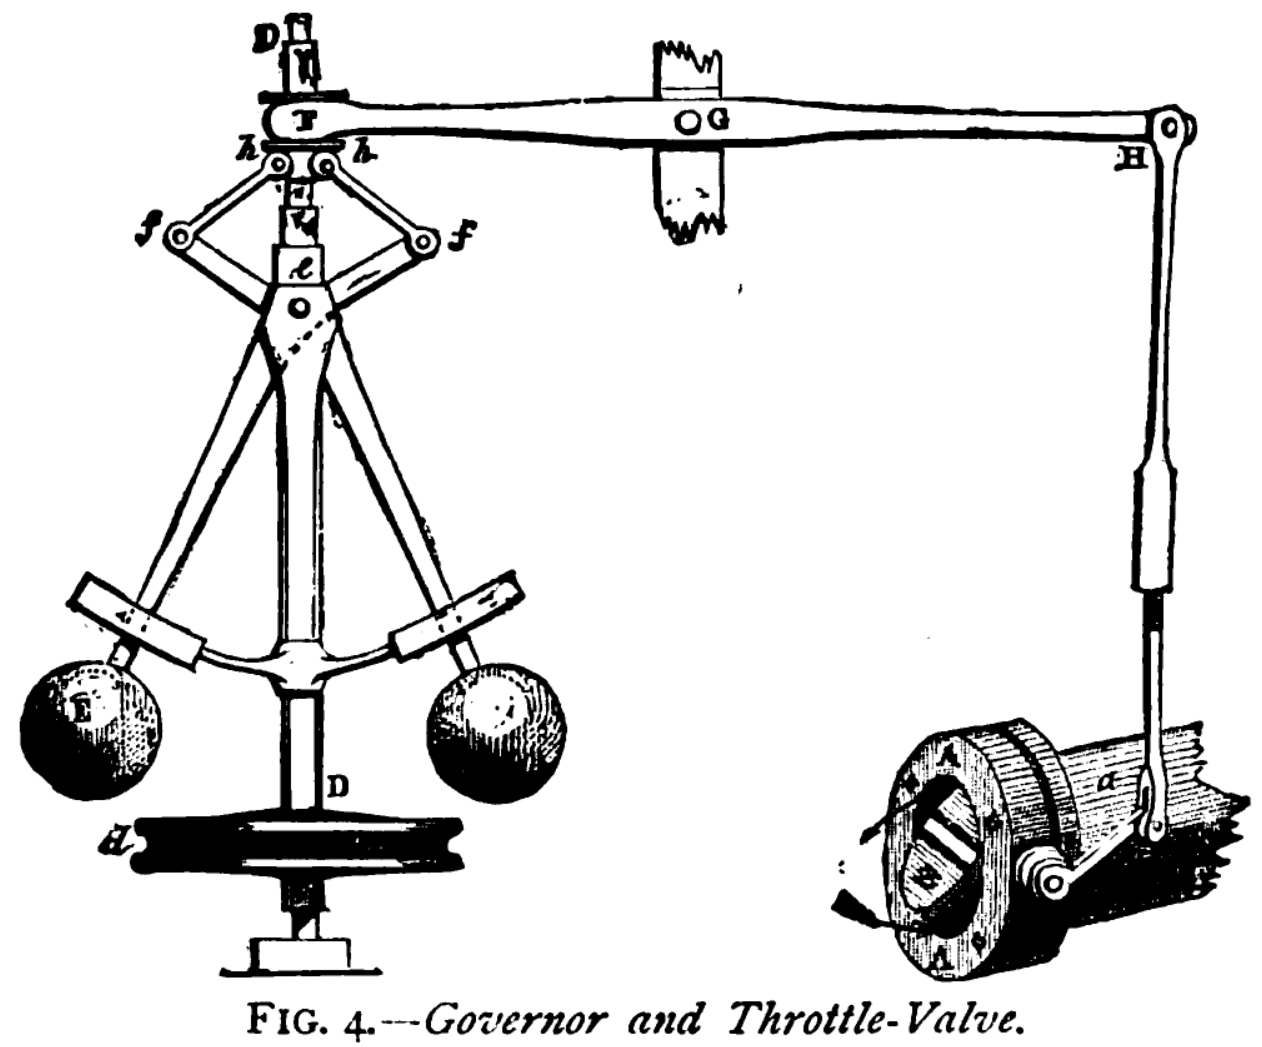
\includegraphics[width=0.7\textwidth]{wattRegulator.png}
    \attribution{R. Siegwart, I.R. Nourbakhsh, Introduction to Autonomous Mobile Robots}
\end{center}

Регуляторы бывают разные:

\begin{itemize}
    \item Релейный регулятор работает очень просто --- если значение больше установочного, пытаемся его уменьшить на фиксированную величину, если меньше, пытаемся увеличить.
        Реализуется как обычный if-then, работает плохо, поскольку реальное значение может бесконечно \enquote{прыгать} около установочного, вообще к нему не приближаясь.
    \item Пропорциональный регулятор: управляющее воздействие пропорционально текущему отклонению от установочного значения.
        То есть, например, чем ближе робот к стене, тем активнее он пытается от неё отъехать, чем дальше --- тем активнее подруливает к стене.
        Это позволяет гораздо более точно управлять системой вблизи установочного значения, но при значительных отклонениях система может сильно \enquote{промахиваться}, и кибернетики даже умеют доказывать теорему, что этот процесс не обязательно сойдётся.
    \item Пропорционально-дифференциальный регулятор: управляющее воздействие пропорционально отклонению от установочного значения и скорости его изменения --- например, если робот слишком быстро отворачивает от стены из-за влияния пропорциональной части, дифференциальная часть заставляет его двигаться плавнее, уменьшая \enquote{перепрыгивание} значения.
    \item ПИД-регулятор: управляющее воздействие пропорционально всему выше и длительности пребывания в ошибочном состоянии --- интегральная часть учитывает историю.
        ПИД-регулятор доказанно сходится, всё ещё довольно прост (имеет всего три коэффициента --- перед пропорциональной, дифференциальной и интегральной частью), поэтому используется повсеместно в реальных задачах, в том числе в качестве элементарного строительного блока для более сложных систем управления.
        Например, делать так, чтобы квадрокоптер висел в воздухе винтами вверх, а не хаотично мотался по сторонам, может ПИД-регулятор, а за целенаправленное движение может отвечать более высокоуровневый автопилот, немного \enquote{возмущающий} ПИД-регулятор в правильном направлении.
\end{itemize}

Поскольку мы не углубляемся в теорию управления, изложение намеренно очень неформально --- если интересно, материалов по регуляторам полно, их изучают на кружках по робототехнике в средней школе.

\subsection{Высокоуровневые системы управления}

Если задача требует чего-то более интеллектуального, регуляторами не обойтись, и могут применяться сколь угодно сложные решения. 
\enquote{Продвинутые} решения условно делятся на два класса, основанные на поведении и основанные на локализации.

Основанные на поведении (Behavior-driven)-решения предполагают, что робот не пытается строить детальной модели мира, а непосредственно реагирует на стимулы (все регуляторы, в общем-то, относятся к этому классу).
Несмотря на кажущуюся простоту, behavior-driven-подход широко распространён и вполне подходит для целого ряда содержательных задач.
Например, боты в компьютерных играх (которые не роботы в смысле этого курса, но сойдут за роботов в симуляторе, плюс-минус симуляция шума сенсоров) часто реализуются именно с behavior-driven-системой управления.

\begin{itemize}
    \item Условие-реакция --- поведение робота определяется набором правил из пары \enquote{условие --- действие, которое надо выполнить, если условие истинно}.
    \item Конечные автоматы --- это то же \enquote{условие-реакция}, но с учётом внутреннего состояния робота и возможностью это состояние менять.
        Конечно-автоматная модель немного сложнее, зато гораздо более гибка, чем \enquote{условие-реакция}, поэтому весьма популярна.
    \item Дерево поведений или дерево задач --- иерархическая структура данных, где во внутренних узлах находятся задачи робота (иерархически уточняющие друг друга), в листьях --- конкретные поведения.
        Активно используется в компьютерных играх, поддержаны в популярных игровых движках, хотя создавались (и, конечно, применяются) в робототехнике.
        По сути дерево поведений можно рассматривать как иерархический конечный автомат, только робот не переходит между состояниями, а выбирает задачи.
        Дерево поведений сложнее всех выше рассмотренных подходов в реализации, но гибче всех, плюс позволяет структурировать код в изолированные строительные блоки и комбинировать из них поведение, зачастую с помощью простой визуальной нотации.
\end{itemize}

Основанные на локализации и планировании --- когда робот строит (или заранее имеет) карту (в более общем случае --- вообще некоторую модель) окружающего мира, пытается определить своё местоположение в этой модели и заранее спланировать свои действия так, чтобы оказаться в желаемом положении.
Тут концептуально есть два подхода:

\begin{itemize}
    \item У нас уже есть карта и набор внешних ориентиров, которые позволяют нам найти на карте себя.
    \item SLAM (Simultaneous Localization And Mapping) --- когда карты изначально нет, мы по данным с сенсоров её строим и одновременно с этим локализуемся.
\end{itemize}

В любом случае у нас должно быть некоторое внутреннее представление карты (что само по себе нетривиальная задача, поскольку окружающий мир непрерывен, а любое представление дискретно) и оценка своей позиции на этой карте (именно оценка, потому что сенсоры врут).
По этим данным можно планировать свои действия, например, прокладывать маршрут по карте обычными графовыми алгоритмами (например, \mintinline{text}{A*}).
В этом деле, естественно, есть масса нюансов, начиная от выбора адекватного задаче представления карты и вероятностного представления верований робота о своём местоположении (оно так и называется в англоязычной литературе, \foreignquote{english}{belief representation}) до ограничений, накладываемых кинематической моделью робота.
Собственно, про нюансы (собственно, и составляющие науку \enquote{робототехника}) мы и поговорим дальше.

\section{Кинематика робота}

Кинематика --- это наука о движении безотносительно того, что это движение вызывает. Применительно к робототехнике кинематика нужна, чтобы уметь отвечать на два вопроса:

\begin{itemize}
    \item Прямая кинематическая задача --- есть кинематическая модель робота и набор управляющих воздействий (на низком уровне, типа \enquote{провернуть колесо на столько-то градусов}), какое положение робот займёт в пространстве?
    \item Обратная кинематическая задача --- есть кинематическая модель робота и целевое положение робота, каков набор управляющих воздействий, необходимых, чтобы целевого положения достигнуть?
\end{itemize}

Под кинематической моделью тут понимается устройство \enquote{движущей части} робота --- его колёсная формула, ведущие/не ведущие, управляемые/не управляемые колёса, число сочленений в манипуляторе или ноге, число и расположение винтов и т.п.
Только для наземных роботов, несколько примеров моделей:

\begin{itemize}
    \item Шагающие --- две ноги, как у людей; четыре ноги, как у животных; 6 ног, как у насекомых.
    \item Колёсные --- четыре известных вида колеса, включая \enquote{шведские} и просто шар в лунке, более десятка широкоизвестных конфигураций этих самых колёс: \enquote{автомобильное} управление, когда два колеса связаны трапециевидным механизмом и синхронно отклоняются в стороны, \enquote{мотоциклетное}, когда есть только одно отклоняемое колесо, дифференциальное (\enquote{танковое}), когда руление выполняется за счёт разности оборотов колёс по разные стороны тележки (обороты вполне могут быть отрицательными, что даёт возможность при такой схеме разворачиваться на месте, в отличие от предыдущих рассмотренных конфигураций), омниколёса (они же шведские колёса, кто ни разу не слышал --- обязательно погуглите), синхропривод.
\end{itemize}

Вот пример кинематической модели, самой хитрой из вышеперечисленных, трёхколёсной синхроприводной тележки:

\begin{center}
    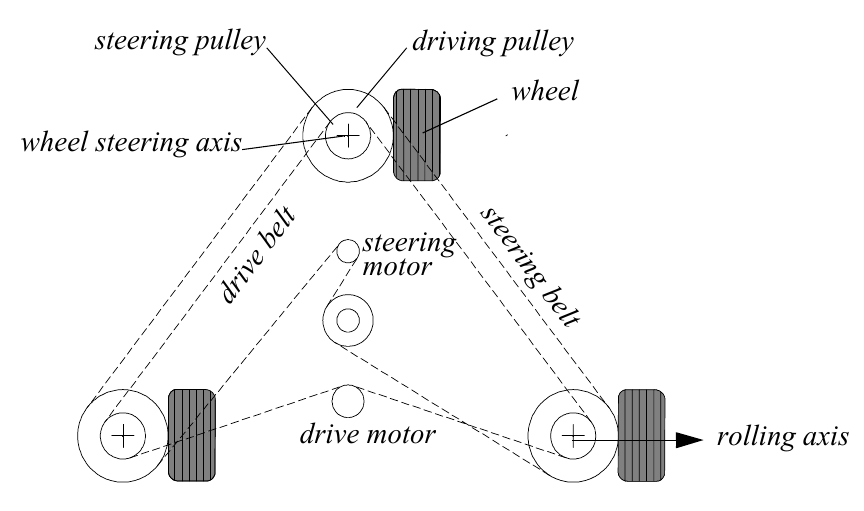
\includegraphics[width=0.7\textwidth]{synchroDrive.png}
    \attribution{R. Siegwart, I.R. Nourbakhsh, Introduction to Autonomous Mobile Robots}
\end{center}

Три колеса управляются двумя моторами, один отвечает за тягу, другой за руление.
Моторы и колёса связаны ременной (или цепной) передачей, что позволяет одному мотору двигать сразу все три колеса.
Схема позволяет поворачивать на месте и довольно точно позиционировать робот, плюс экономить дорогие моторы, но механически сложна, поэтому редко используется.

Например, бытовые роботы-пылесосы в подавляющем большинстве случаев представляют собой трёхколёсные тележки с дифференциальным управлением с двумя ведущими колёсами и одним пассивным (не связанным с мотором) поворотным колесом.

У каждой кинематической модели есть степени свободы --- сколько независимых параметров описывают состояние модели.
Не всегда всеми ими можно управлять.
Например, робот на омниколёсах может независимо менять свои координаты по любой из осей и своё положение в пространстве, у него три степени свободы и все три управляемы.
Робот с автомобильным управлением (например, беспилотный автомобиль) может двигаться вперёд-назад и отклонять рулевые колёса (так что мы управляем двумя переменными из трёх).
Для роботов-манипуляторов степени свободы --- это количество сочленений и степени свободы шарниров, для шагающих роботов --- тоже, но даже если мы можем всеми сочленениями управлять независимо, есть естественное ограничение, что робот не должен упасть, так что фактически управляемых степеней свободы у него принципиально меньше, чем степеней свободы вообще.

Роботы, у которых мы можем управлять всеми их степенями свободы, называются \emph{голономными}, если нет --- соответственно \emph{неголономными}.
Понятие голономности в математике более общо и определяется интегрируемостью уравнений, но в робототехнической кинематике это на самом деле оказывается эквивалентным простому определению выше.

Формально для обсуждения кинематики вводится понятие \emph{позы робота}, то есть расположения его в пространстве.
Например, для трёхколёсной тележки поза описывается координатами в двумерном пространстве и углом поворота робота:

\begin{center}
    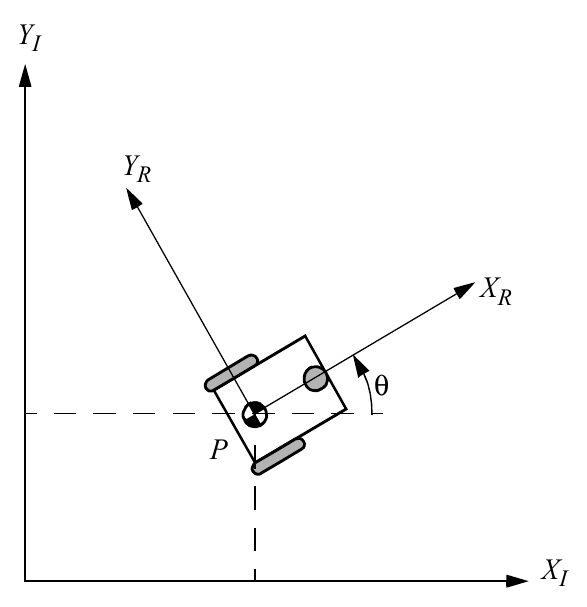
\includegraphics[width=0.7\textwidth]{pose.png}
    \attribution{R. Siegwart, I.R. Nourbakhsh, Introduction to Autonomous Mobile Robots}
\end{center}

Для летающих роботов всё несколько сложнее, для манипуляторов даже ещё интереснее.

Поза всегда оценивается относительно некоторой глобальной системы координат, формально в виде вектора
$$\xi_I = \begin{bmatrix} x \\ y \\ \theta \end{bmatrix}$$

Тогда кинематическая модель робота формально может быть формально описана как функция от 

\item Прямая кинематическая модель:
        $$\dot{\xi_I} = \begin{bmatrix} \dot{x} \\ \dot{y} \\ \dot{\theta} \end{bmatrix} = f(l, r, \theta, \dot{\phi_1}, \dot{\phi_2})$$
    \item Каждая модель накладывает ограничения на возможные движения
\end{itemize}
\end{column}
\begin{column}{0.4\textwidth}

\end{document}
